\chapter{Die Vierträgerzelle: ein gemeinsames Muster}
\label{ch:zelle}
\section{Ein Zustand, dessen Teile allein nichts verraten}
Vier Träger mit je vier Basiswerten besitzen den total antisymmetrischen Zustand
\begin{equation}
\ket\Omega=\frac1{\sqrt{24}}\sum_{\pi\in S_4}\operatorname{sgn}(\pi)
\ket{\pi(0)\pi(1)\pi(2)\pi(3)}.
\label{eq:omega}
\end{equation}
Jedes Basiswort verwendet alle vier Werte genau einmal. Die 24 Permutationen erhalten passende Vorzeichen. Das Ergebnis ist ein reiner gemeinsamer Zustand. Jeder einzelne Träger sieht für sich trotzdem maximal gemischt aus:
\begin{equation}
\rho_i=I_4/4,\qquad \rho_{ij}=(I_{16}-S_{ij})/12.
\end{equation}
Die Paarreduktion hat Rang sechs und sechs gleich große Eigenwerte $1/6$. Die Ordnung steckt in den Beziehungen zwischen den Teilen. \src{S08, §3; S01--S03}

\begin{figure}[H]\centering
\begin{tikzpicture}
\foreach \n/\x/\y in {1/0/0,2/3/0,3/0/2.5,4/3/2.5}{\node[box,circle,minimum size=13mm] (n\n) at (\x,\y) {$\n$};}
\foreach \a/\b in {1/2,1/3,1/4,2/3,2/4,3/4}{\draw[teal,thick] (n\a)--(n\b);}
\node[box,text width=58mm] at (8,1.25) {Jeder einzelne Träger: $I_4/4$\\Jedes Paar: antisymmetrisch\\Gemeinsam: reines Singulett $\Omega$};
\end{tikzpicture}
\caption{Die vollständige Vierergraph-Zelle. Die Linien bezeichnen im Hamiltonmodell Paarwechselwirkungen. Sie sind keine bereits hergeleiteten Raumrichtungen.}
\end{figure}

\section{Der Hüllensatz und seine genaue Voraussetzung}
Sei $P^+_{ij}=(I+S_{ij})/2$ der Projektor auf den symmetrischen Paarraum. Wenn für alle Paare $P^+_{ij}\psi=0$ gilt, dann hat jeder Swap Eigenwert minus eins. Da Transpositionen alle Permutationen erzeugen, folgt
\begin{equation}
\psi\in\Lambda^N\C^4.
\end{equation}
Für $N=4$ ist dieser Raum eindimensional, für $N\ge5$ null. Auch gemischte Zustände mit entsprechender Trägerbedingung erfüllen die Aussage. Für $N=1,2,3$ existieren aber ebenfalls antisymmetrische Zustände. Vier ist daher die maximale Besetzung und die erste eindeutige Singulettgröße unter diesen Bedingungen; eine Auswahl „die Natur muss genau vier nehmen“ folgt erst mit einer zusätzlichen Anforderung.

Ein stärkerer Graphsatz benötigt die Bedingung nur entlang eines zusammenhängenden Graphen:
\begin{equation}
H_\Gamma=\sum_{(i,j)\in E(\Gamma)}J_{ij}P^+_{ij},\quad J_{ij}>0
\quad\Longrightarrow\quad\ker H_\Gamma=\Lambda^N\C^4.
\end{equation}
Die Kantentranspositionen eines zusammenhängenden Graphen erzeugen die gesamte symmetrische Gruppe. Nullenergie in einer Summe positiver Operatoren verlangt Nullenergie jedes Terms. Damit ist der Satz bewiesen.

\section{Eine weiche Energiebedingung erlaubt Bewegung}
Das vollständige Tetramermodell lautet
\begin{equation}
H_{\mathrm{tet}}=J\sum_{1\le i<j\le4}P^+_{ij},\qquad J>0.
\end{equation}
Es besitzt das exakte Spektrum
\begin{equation}
\spec(H_{\mathrm{tet}}/J)=\{0^{[1]},2^{[45]},3^{[40]},4^{[135]},6^{[35]}\}.
\label{eq:tet-spec}
\end{equation}
Der Grundzustand ist $\Omega$, die Lücke $2J$. Die hochgestellten Zahlen zählen die Zustände pro Energiewert und summieren sich zu 256.

Ein hartes Verbot aller symmetrischen Paaranteile lässt dagegen nur $\C\Omega$ übrig. Ein lokaler Tick erzeugt im Quellprotokoll gerade solche Anteile, nämlich $\langle P^+_{1j}\rangle=5/8$. Er wäre im hart eingeschränkten Raum unzulässig. Für Dynamik braucht man deshalb eine weiche Energiestrafe, zusätzliche Sektoren oder eine andere Kompositionsregel. In der weichen Lesart ist $J$ ein Energiemaß und nicht bloß ein bedeutungsloser Strafparameter.

Dass $\mathrm{Sym}^2(4)=10$ in der betreffenden Zerlegung der adjungierten $E_8$-Algebra fehlt, beweist kein Verbot symmetrischer Zustände im Tensorprodukt physischer Träger. Generatorraum, Zustandsraum und Klammerziel sind verschiedene Dinge. Der Hüllensatz bleibt richtig; die physikalische Herkunft seiner linken Voraussetzung ist offen.

\section{Was ein Zustand über seinen Generator verrät}
Der vollständige Graph, ein Stern und ein Pfad besitzen auf vier Trägern denselben antisymmetrischen Grundzustand, aber verschiedene Anregungen. Für gleiche Sterngewichte ist die Lücke $J/2$ statt $2J$. S01 nennt für einen Pfad mit Gewichten $1,2,3$ etwa $0{,}467911$; S06 für sechs Gewichte $1,2,3,4,5,6$ etwa $3{,}847309$. Die letzten Werte werden hier als Quellnumerik übernommen.

\begin{bild}{Ein Tiefpunkt verrät nicht die Form des ganzen Tals}
Man kennt den tiefsten Punkt einer Landschaft. Daraus weiß man noch nicht, ob der Weg dorthin steil, flach oder von mehreren Hügeln umgeben ist. Ebenso bestimmt der Grundzustand nicht sämtliche Kopplungen und Anregungsenergien seines Hamiltonoperators.
\end{bild}

Ein nützliches robustes Zustandszertifikat folgt dennoch aus der Tetramerlücke:
\begin{equation}
H_{\mathrm{tet}}\ge2J(I-\ket\Omega\bra\Omega),\qquad
1-\bra\Omega\rho\ket\Omega\le\frac12\sum_{i<j}\langle P^+_{ij}\rangle.
\end{equation}
Kleine gemessene Paarenergien garantieren Nähe zum Zustand. Sie zertifizieren nicht automatisch den Generator oder seine Herkunft.

\section{Warum Austausch allein die Zelle nicht herstellt}
\begin{bild}{Integrierte Vereinfachung v1.6: ein Record genügt im Laborvertrag}
Die folgende Austausch-Erhaltungsgrenze bleibt richtig. Neu ist aber ein expliziter Stabilizer-Eingang $\xi$, für den eine einzige antisymmetrische Record-Auswahl exakt $\Omega$ erzeugt:
\[
P^-_{03}\ket\xi=-\sqrt{3/8}\ket\Omega.
\]
Die Erfolgswahrscheinlichkeit beträgt $3/8$, nicht eins. Der kohärente Record bleibt eine zusätzlich bereitzustellende Ressource; er ist nicht bloß ein Clifford-Gate. Lange Näherungsfilter sind für \emph{dieses} Präparationsziel innerhalb \emph{dieses} Ressourcenvertrags nicht mehr nötig. Die vollständige Einordnung einschließlich Schlussprüfung und Misserfolgen steht in Kapitel~\ref{ch:v16-labor}.
\end{bild}


Der Projektor $A_4=\ket\Omega\bra\Omega$ kommutiert mit allen Swaps. Daher erhält jede rein zellinterne Austauschentwicklung, auch mit zeitabhängigen Gewichten, den Anteil $\Tr(A_4\rho)$. Kollektive $\mathrm{SU}(4)$-Drehungen tun dasselbe. Ein Grundzustand kann also bekannt sein, ohne dass der vorhandene Ablauf einen beliebigen Eingang dorthin bringt.

Die konkrete Präparation in Kapitel~\ref{ch:echo} ergänzt dafür ausdrücklich weitere Operationen. Dort wird auch gezeigt, weshalb ein reiner Clifford-Baukasten nicht ausreicht.

\chapter{Vermittlung und Graph: die Prüfung der fünf Fugen}
\label{ch:fugen}
\begin{bild}{Aktualisierung v1.5: ein exakter kleinerer Spektralauftrag}
Der 80-dimensionale Standard-Multiplizitätsblock ist inzwischen explizit konstruiert und sein einfaches Spektrum exakt zertifiziert. Eine zusätzliche Tableau-Transposition reduziert die führenden Singulettprobleme auf höchstens 131-dimensionale quadrierte Singularwertprobleme. Das beweist noch keine globale Ordnung aller SU(4)-Sektoren. Siehe Kapitel~\ref{ch:spectrum15}.
\end{bild}
\section{Wie ein virtueller Zwischenzustand bindet}
Der gewünschte positive Austausch lässt sich in einem kleinen Modell genau erklären. Man ergänzt den Paarraum $\C^4\otimes\C^4$ durch einen sechsdimensionalen Vermittler mit Energie $\Delta>0$. Die partielle Isometrie $W$ erfüllt
\begin{equation}
W^\dagger W=P_-=(I-S)/2,\qquad WW^\dagger=I_6.
\end{equation}
Für
\begin{equation}
H=\begin{pmatrix}0&gW^\dagger\\gW&\Delta I_6\end{pmatrix}
\end{equation}
bleiben die zehn symmetrischen Zustände bei null; die antisymmetrischen Zustände koppeln paarweise an den Vermittler. Die unteren Energien sind
\begin{equation}
E_-^{\mathrm{med}}=\frac{\Delta-\sqrt{\Delta^2+4g^2}}2.
\end{equation}
Nach Identifikation des angekleideten niedrigen Bands und einer gemeinsamen Energieverschiebung entsteht exakt
\begin{equation}
H_{\mathrm{eff}}=J_{\mathrm{eff}}P_+,\qquad
J_{\mathrm{eff}}=\frac{\sqrt{\Delta^2+4g^2}-\Delta}{2}
=\frac{g^2}{\Delta}-\frac{g^4}{\Delta^3}+\cdots.
\end{equation}
\src{S01, §3; S05, §7}

Bildhaft sinkt die antisymmetrische Kombination im Energievergleich ab, weil sie eine zusätzliche virtuelle Ausweichmöglichkeit besitzt. Das liefert ein positives relatives Gewicht der symmetrischen Kombination. Bei symmetrischen Vermittlern kommt eine konkurrierende Absenkung hinzu. Das Vorzeichen ist dann nicht allein durch den Namen $E_8$ bestimmt.

Die allgemeine kontrollierte Elimination hoher Energien gehört zur Schrieffer-Wolff-Methode. Hier ist der einzelne 22-dimensionale Baustein direkt lösbar. Das macht ihn zu einer guten Gegenprobe für eine spätere native Kopplung, ersetzt aber nicht deren Auswahl. \href{https://arxiv.org/abs/1105.0675}{Bravyi, DiVincenzo und Loss [E2]}

\begin{grenze}{Vermittlungskorrektur v1.3}
Für $K\ket{ab}=-K\ket{ba}$ müssen die beiden Anordnungen innerhalb einer Kante kohärent bleiben. Orthogonale Records für $ab$ und $ba$ ersetzen $I-S$ durch $I-D$ und zerstören den gewünschten Austausch. Verschiedene Kanten dürfen durch Loch- und Zuschauerzustände unterscheidbar bleiben. Kapitel~\ref{ch:audit13} rechnet die korrigierte Ausführung und ihre vierte Ordnung aus.
\end{grenze}
\section{Der Clebsch-Vorschlag: eine genaue neue Graphlesart}
S11 macht die zusätzliche Zuordnung: Ein $D_5$-Spinorgewicht $s$ ist ein Ort; das $A_3$-Gewicht $a$ ist der lokale Viererzustand. Die 64 Gewichte von $(16,4)$ werden somit als 16 Orte mit je vier inneren Zuständen gelesen. Das ist eine konkrete \status{bedingte} Interpretation, keine bloße Umbenennung einer bereits gegebenen räumlichen Geometrie.

Schreibe die 16 Spinorgewichte als $(\pm\frac12)^5$ mit fester Vorzeichenparität. Zwei Orte sind Nachbarn, wenn sie sich in vier der fünf Vorzeichen unterscheiden. Dann ist $s+s'$ ein Vektorgewicht $\pm e_i$. Der entstehende Graph besitzt
\begin{equation}
16\text{ Knoten},\quad40\text{ Kanten},\quad\deg=5,\quad
\spec A_\Gamma=\{5^{[1]},1^{[10]},(-3)^{[5]}\}.
\end{equation}
Er ist der Clebsch-Graph, stark regulär mit Parametern $(16,5,0,2)$, dreiecksfrei und nicht bipartit. Die fünf Vorzeichenkoordinaten teilen seine Kanten in fünf perfekte Matchings. Die zehn Bindungslabels $\pm e_i$ tragen je vier Kanten. Diese Eigenschaften wurden hier mit ganzzahligen Gewichten und einer exakten charakteristischen Polynomprüfung unabhängig bestätigt.

\begin{figure}[H]\centering
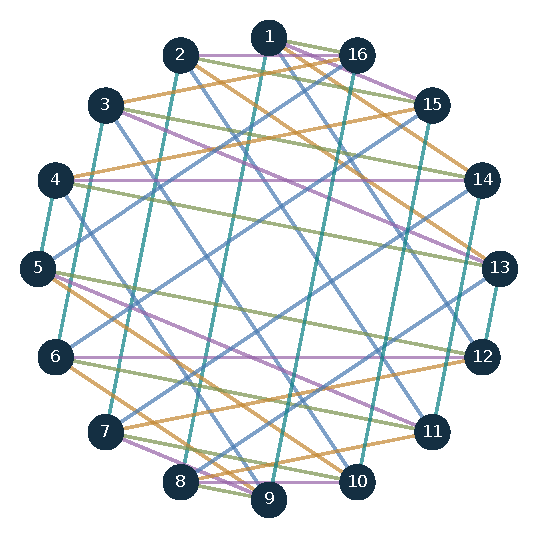
\includegraphics[width=.8\linewidth]{figures/clebsch.pdf}
\caption{Der bedingte Clebsch-Kopplungsgraph. Farben kennzeichnen die fünf perfekten Matchings. Die Kreispositionen und Knotennummern sind nur Zeichnungskonventionen; sie behaupten keine räumliche Einbettung oder physikalische Entfernung.}
\end{figure}

Der gleichgradige Klammerkanal ist auf dem Viererfaktor antisymmetrisch. Bei der in S11 gewählten Normierung $K^\dagger K=I-S=2P_-$ ergibt eine \emph{zusätzlich angenommene} einheitliche Vermittlerenergie und Amplitude in zweiter Ordnung
\begin{equation}
H_{\mathrm{eff}}=-\frac{t^2}{\Delta}K^\dagger K
=\frac{2t^2}{\Delta}P_++\text{Konstante}.
\end{equation}
Der Faktor zwei gegenüber dem vorigen $W$-Modell liegt in der Normierung: $K=\sqrt2W$, entsprechend $g=\sqrt2t$.

\section{Welche Auswahl hier noch hinzukommt}
Die Graphkombinatorik folgt aus der angegebenen Ortslesart. Um daraus einen Vielteilchen-Hamiltonoperator zu erhalten, braucht man außerdem eine Fock- oder Tensorproduktstruktur, Besetzungsbedingungen, die Bedeutung der virtuellen Zustände und ihre Energien. Betragsgleiche Chevalley-Strukturkonstanten wählen noch keine physikalischen Kopplungsstärken in normierten Mehrteilchenzuständen aus. Gleiche $t$ und $\Delta$ müssen dynamisch oder durch eine entsprechend starke Symmetrie des \emph{gesamten} Modells begründet sein.

Auch das Wort „hard-core“ folgt nicht allein aus einer fehlenden Wurzelsumme. Für zwei verschiedene lokale $A_3$-Gewichte am selben Spinorgewicht beträgt das Normquadrat der gesamten Summe sechs; bei gleichem Gewicht acht. Die fünf in S11 sind der $D_5$-Anteil allein. In beiden Fällen ist die Summe zwar keine Wurzel der Norm zwei. Daraus folgt zunächst nur das Fehlen dieses direkten Klammerkanals, keine automatisch verbotene Doppelbesetzung eines noch zu definierenden Fockraums.

Da ein Vektorlabel vier Kanten trägt, muss die effektive Rechnung zudem erklären, wie virtuelle Zustände verschiedenen Bindungen zugeordnet werden. Identische reine Vermittlerlabels können in einem bloßen Zwei-Teilchen-Modell Kreuzterme erzeugen. In einem fest besetzten Vielteilchenraum können verschiedene Loch- und Zuschauerzustände sie dagegen unterscheiden. Genau diese noch offene Belegungsstruktur entscheidet, ob nur der behauptete Paarterm bleibt.

Der Clebsch-Graph enthält keinen vollständigen $K_4$. Daraus folgt nicht, dass der Zustand $\Omega$ unmöglich wäre: Ein verbundener Viererpfad reicht für denselben Kern. Es folgt aber, dass der vollständige Tetramer-Hamiltonoperator nicht einfach die induzierte native Viererstruktur dieses Graphen ist. Ebenso macht uniforme Clebsch-Kopplung daraus keine uniforme Kette. Der Schluss „also $\lambda=J$ in der Kette und damit WZW“ wechselt den Graphen und benötigt einen eigenen Nachweis.

\section{Die berichteten Clusterzahlen}
\par\noindent\begin{tabularx}{\linewidth}{L{74mm}Y}
\toprule
\textbf{Clebsch-Cluster bei $J=1$, nach S11}&\textbf{Berichteter Wert}\\\midrule
Grundenergie&$11{,}045398$\\
Grundzustand&Eindeutiges $\mathrm{SU}(4)$-Singulett, Form $(4,4,4,4)$\\
Erster angeregter Singulettwert&$11{,}561762$; mindestens vier orthogonale Moden, Gap etwa $0{,}516$\\
Erste adjungierte Anregung&$12{,}133537$, Gap etwa $1{,}088$\\
Weitere Multiplets&$20'$ bei $12{,}3228$; $45$ bei $12{,}8751$ und $12{,}9816$\\
Symmetrisches Gewicht pro Kante&$0{,}27613$\\
Symmetrisches Gewicht pro Nichtkante&$0{,}61193$\\
Summe über alle 120 Paare&$60$\\
Produkt aus vier disjunkten $\Omega$-Viererzyklen&$15J$, im Text zugleich als untere Schranke aller solchen Produktformen angegeben\\\bottomrule
\end{tabularx}\par
Die vollständige Clusterdiagonalisierung wurde hier nicht wiederholt. Es handelt sich um numerische Eigenwerte aus S11, nicht um exakte algebraische Eigenzahlen. Die Graphidentitäten sind unabhängig exakt bestätigt; das ist eine andere Evidenzklasse. Ein Rang oder eine Darstellung kann exakt feststehen, während ihre Eigenwerte numerisch berechnet werden.

\begin{grenze}{Neue Singulettprüfung v1.3}
Zwei zusätzliche Läufe im vollen 24024-dimensionalen Singulett-Multiplizitätsraum finden mindestens vier orthogonale Moden bei $11{,}561762122803J$, mit Residuen unter $10^{-8}$. Das alte Dublett ist korrigiert. Eine exakte obere Multiplizitätsschranke und ein neuer Lauf aller Nichtsingulettsektoren fehlen. Die übrigen Tabellenwerte bleiben S11 zugeschrieben.
\end{grenze}
\section{Neue Korrektur: Singulett heißt nicht eindeutig}
S11 behauptet für den \emph{vollständigen} Graphen mit $N=4m$ einen eindeutigen Grundzustand bei $E_0=5m(m-1)J$ und Gap $2J$. Energie und Gap stimmen; die Eindeutigkeit stimmt ab acht Trägern nicht.

Der Hamiltonoperator ist dort die zentrale Transpositionssumme. Auf der Youngform $\lambda=(m,m,m,m)$ wirkt $\mathrm{SU}(4)$ trivial, aber diese Darstellung tritt mit der Specht-Multiplizität $f^\lambda$ auf. Der Grundraum hat deshalb
\begin{equation}
\dim\mathcal H_0=f^{(m,m,m,m)}
=\frac{(4m)!}{\prod_{(r,c)\in(m^4)}h_{rc}}.
\end{equation}
\begin{center}
\begin{tabular}{rrrr}
\toprule $N$&$E_0/J$&Gap$/J$&Grundraumdimension\\\midrule
4&0&2&1\\8&10&2&14\\12&30&2&462\\16&60&2&24024\\\bottomrule
\end{tabular}
\end{center}
Diese Werte wurden hier durch Enumeration aller Youngformen mit höchstens vier Zeilen und exakte Hookformeln geprüft; die gesamten Schur-Weyl-Dimensionen ergeben jeweils $4^N$. Das ist eine konkrete Korrektur des vollständigen Graphen. Sie widerlegt nicht die separat berichtete numerische Eindeutigkeit des Clebsch-Grundzustands, dessen Hamiltonoperator nicht dieselbe zentrale Summe ist.

\section{Neue Präzisierung: Aufzeichnung ist nicht durch die 248 verboten}
\textbf{Operatoren unterscheiden (v1.3):} Das folgende $Q=I-2D$ beschreibt eine gleichkontextige Vierer-Aufzeichnung. Das neue binäre Austauschregister $R=P_+\otimes I+P_-\otimes X$ ist ein anderer Operator und nachweislich nicht Clifford. Seine zusätzliche Ressourcenanforderung widerspricht der folgenden Darstellbarkeit von $Q$ nicht.

Die Sektortrennung aus S11 ist für die \emph{gleichkontextige} Kopplung anschaulich: $Q$ reflektiert den von $\ket{jj}$ aufgespannten Vierraum, der in $\mathrm{Sym}^2(4)$ liegt. Auf $\Lambda^2(4)$ wirkt es als Identität. Entsprechend lässt dieser spezielle Operator den Paaranteil einer idealen $\Omega$-Zelle unverändert. Bei einer anderen Registerbasis gilt die Aussage nicht automatisch; S11 berichtet dafür $1/15$ statt $15/15$ Kontexte.

Der daraus gezogene Schluss „eine Cross-Register-Aufzeichnung ist innerhalb der 248 unmöglich“ geht jedoch über den bewiesenen Satz hinaus. Ein Tensorprodukt von Trägern und zusammengesetzte Operatoren sind nicht auf die irreduziblen \emph{Generatorbestandteile} der Adjungierten beschränkt.

Ein expliziter Gegenbeleg im vorhandenen Vierer-Matrixbaukasten verwendet
\begin{equation}
D=\sum_{j=0}^3\ket{jj}\bra{jj}
=\frac14\left(I\otimes I+Z_1\otimes Z_1+Z_2\otimes Z_2
+Z_1Z_2\otimes Z_1Z_2\right),
\end{equation}
wobei $Z_1,Z_2$ die beiden Pauli-$Z$ im Viererträger sind. Dann gilt
\begin{equation}
Q=I-2D=e^{-i\pi D},\qquad Q^2=I.
\end{equation}
Diese Operatoridentitäten und die Wirkung auf den antisymmetrischen Sektor wurden hier exakt geprüft. Die lokale Matrixalgebra samt zugelassener trägerübergreifender Produkte kann die Kopplung also ausdrücken.

\begin{grenze}{Was dadurch gelöst ist und was offen bleibt}
Gelöst ist die algebraische Darstellbarkeit nach Zulassung einer konkreten Tensorproduktkopplung. Nicht gelöst ist ihre physikalische Verfügbarkeit aus der primitiven TFPT-Quelle. Ein größerer $E_8$-Modul wie die in S11 vorgeschlagene 3875 kann ein möglicher Forschungsweg sein; seine Notwendigkeit folgt nicht aus dem Sektorargument. Die dort genannte Verzweigung und ein tatsächlich geeigneter Aufzeichnungsoperator in diesem Modul sind hier nicht geprüft.
\end{grenze}
